\subsubsection{06.12.14}

\begin{enumerate}
	\item Время начала и окончания собрания:
	16:10 - 20:10
	\item Цели собрания:
	\begin{enumerate}
	  \item Создать чертеж нового ковша.
	  
	  \item Выбрать материал, из которого мы будем изготавливать ковш.
	  
    \end{enumerate}
	\item Проделанная работа:
	\begin{enumerate}
	  \item Была разработана развертка ковша.
	  
	  \begin{figure}[H]
	  	\begin{minipage}[h]{0.2\linewidth}
	  		\center  
	  	\end{minipage}
	  	\begin{minipage}[h]{0.6\linewidth}
	  		\center{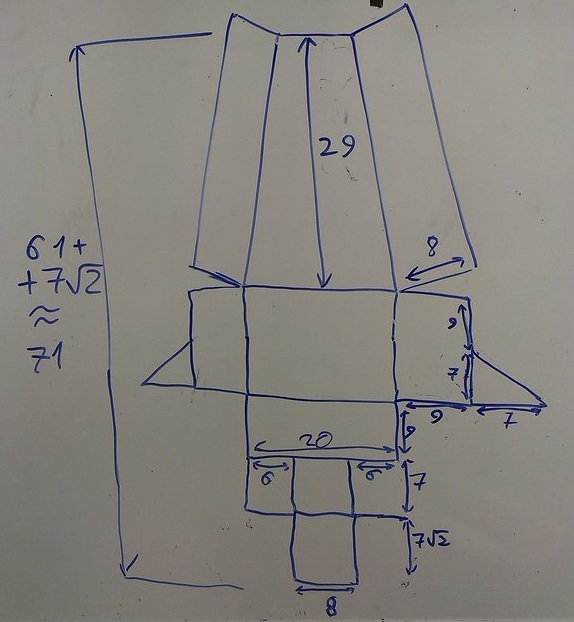
\includegraphics[scale=0.3]{days/06.12.14/images/01}}
	  		\caption{Чертеж развертки ковша с расстоянием в см}
	  	\end{minipage}
	  \end{figure}
	  
	  \item Было решено использовать для создания ковша листовой пластик ПЭТ (такой, из которого изготавливаются бутылки).
	  
	  \item Во время тренировок с раздвиганием подъемника мы заметили, что механизм лебедки немного шатается, что не сказывается на его работе, но может привести к разбалтыванию винтов. Для того, чтобы упрочнить конструкцию, мы добавили поперечное ребро жесткости.
	  
	  \begin{figure}[H]
	  	\begin{minipage}[h]{0.2\linewidth}
	  		\center  
	  	\end{minipage}
	  	\begin{minipage}[h]{0.6\linewidth}
	  		\center{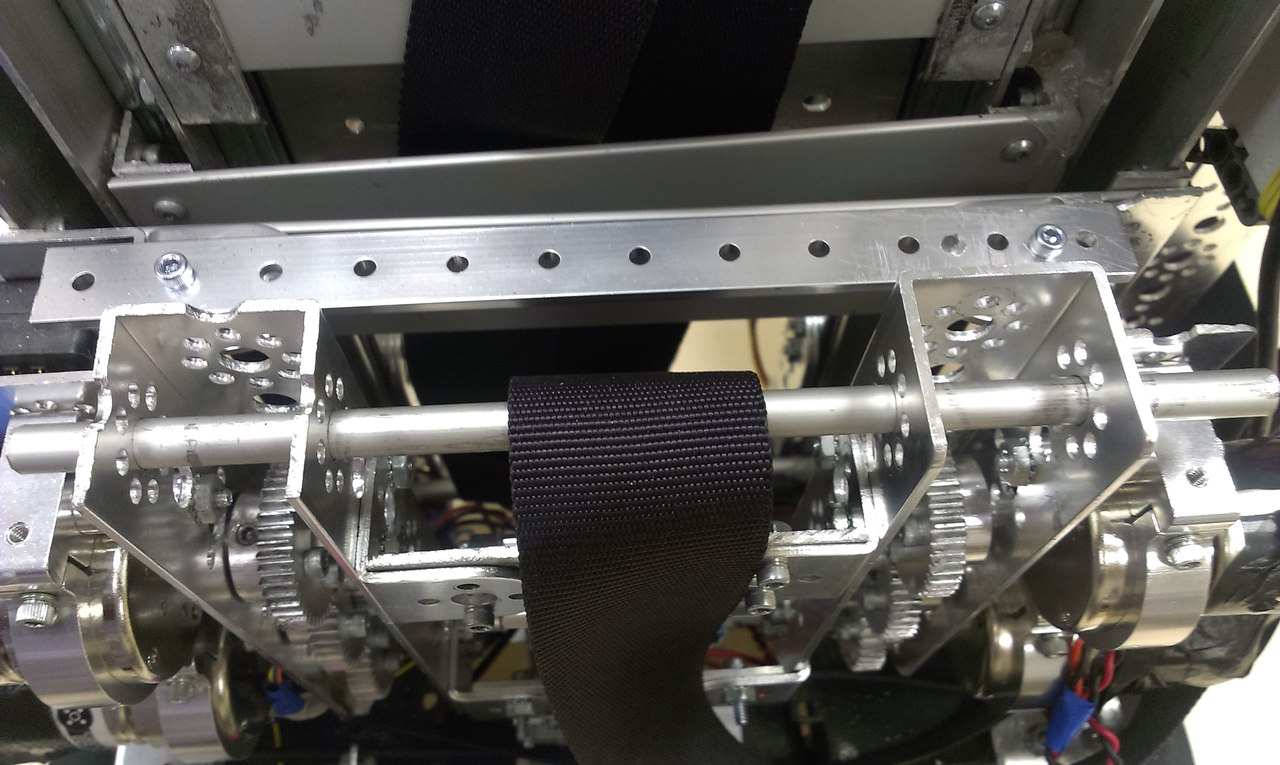
\includegraphics[scale=0.2]{days/06.12.14/images/02}}
	  		\caption{Ребро жесткости}
	  	\end{minipage}
	  \end{figure}
	  
    \end{enumerate}
    
	\item Итоги собрания: 
	\begin{enumerate}
	  \item Развертка ковша разработана.
	  
	  \item Материал для ковша выбран.
	  
	  \item Лебедка упрочнена.
	  
    \end{enumerate}
    
	\item Задачи для последующих собраний:
	\begin{enumerate}
	  \item Выкроить из пластика развертку ковша и склеить его.
	  
    \end{enumerate}     
\end{enumerate}
\fillpage